\documentclass[10pt]{beamer}

\usetheme[progressbar=frametitle]{metropolis}
\usepackage{appendixnumberbeamer}

\usepackage{booktabs}
\usepackage[scale=2]{ccicons}
\usepackage{caption}
\captionsetup{justification=raggedright, singlelinecheck=true}
\usepackage{subfig}
\captionsetup[subfloat]{labelformat=empty}

\usepackage{xspace}
\newcommand{\themename}{\textbf{\textsc{metropolis}}\xspace}


\usepackage[bookmarksopen=true]{hyperref}
\usepackage{xcolor}
\usepackage{graphicx}
\usepackage[group-separator = {,}]{siunitx}

\newcommand{\faro}[0]{FARO\textsuperscript{\textregistered}\space}
\newcommand{\farons}[0]{FARO\textsuperscript{\textregistered}}

% Use metropolis theme
\title{Hyper Parameter Optimization \newline using Machine Learning}
\date{July, 2021}
\author{{Nuno Costa} \texorpdfstring{ \\
{\textit{ISEP Advisor}: Carlos Ramos} \newline
{\textit{External Advisor}: Hooshiar Zolfagharnasab}}{}}
\institute{Polytechnic of Porto - School of Engineering (ISEP)}


\begin{document}

  \maketitle
  \section{Introduction}
  \begin{frame}{\faro Overview}
    \vspace{1cm}
    \begin{columns}
      \begin{column}{0.7\textwidth}
          \faro is a leader in the 3D metrology market 

          Over US \$ 150 M gross profit in 2020

          Sells hardware devices and software solutions
      \end{column}
      \begin{column}{0.3\textwidth}
        \begin{figure}
        \centering
        
\includegraphics[width=\textwidth]{images/faro_logo.png}
        \end{figure}
      \end{column}
    \end{columns}
    \begin{columns}
      \begin{column}{0.30\textwidth}
        \begin{figure}
          \centering
          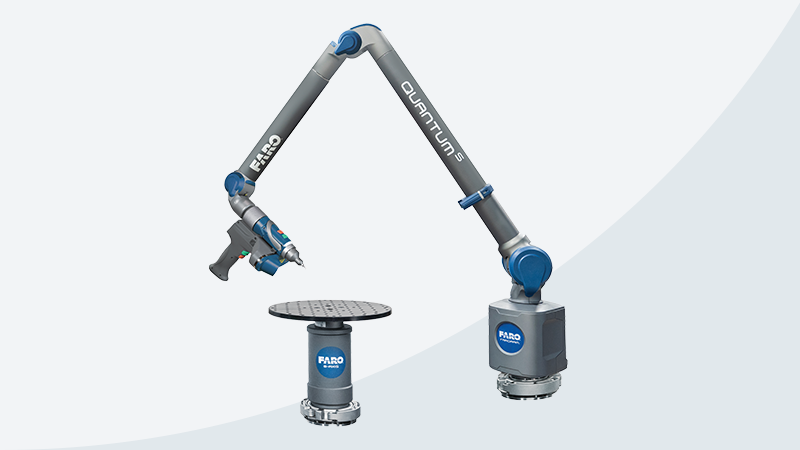
\includegraphics[width=\textwidth]{images/faro_quantum_s_arm.png}
          \caption*{\faro Quantum Max \newline Scan Arm}
        \end{figure}
      \end{column}
      \begin{column}{0.30\textwidth}
        \begin{figure}
          \centering
          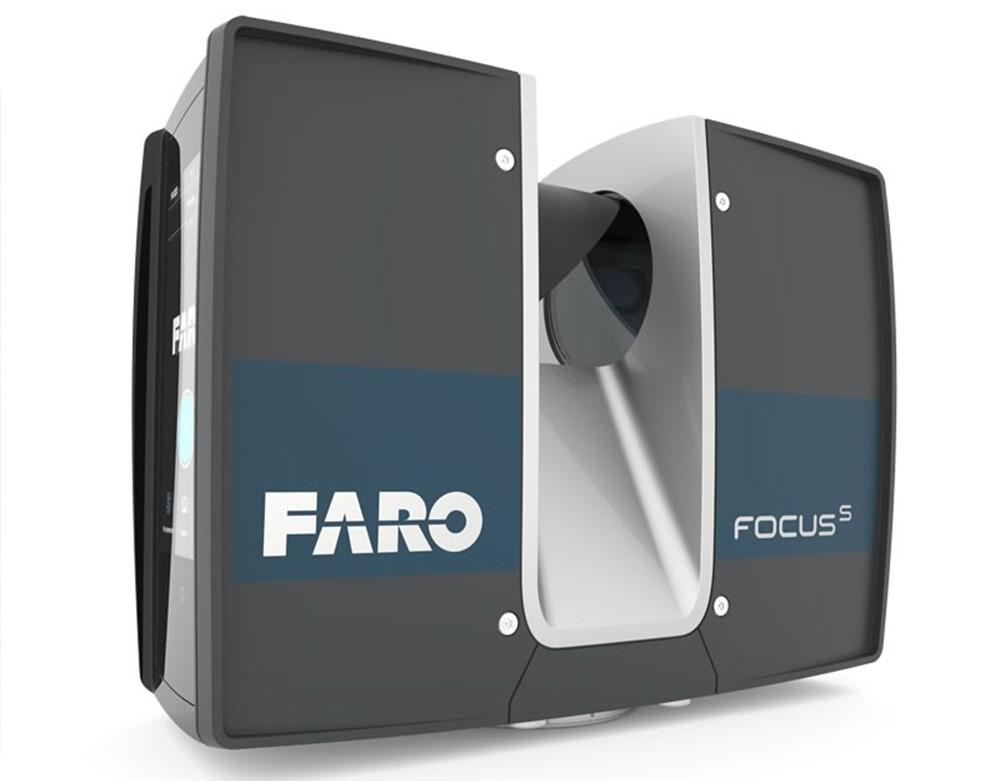
\includegraphics[width=\textwidth]{images/faro_scanner.jpg}
          \caption*{\faro Focus \newline Laser Scanner}
        \end{figure}
      \end{column}
      \begin{column}{0.30\textwidth}
        \begin{figure}
          \centering
          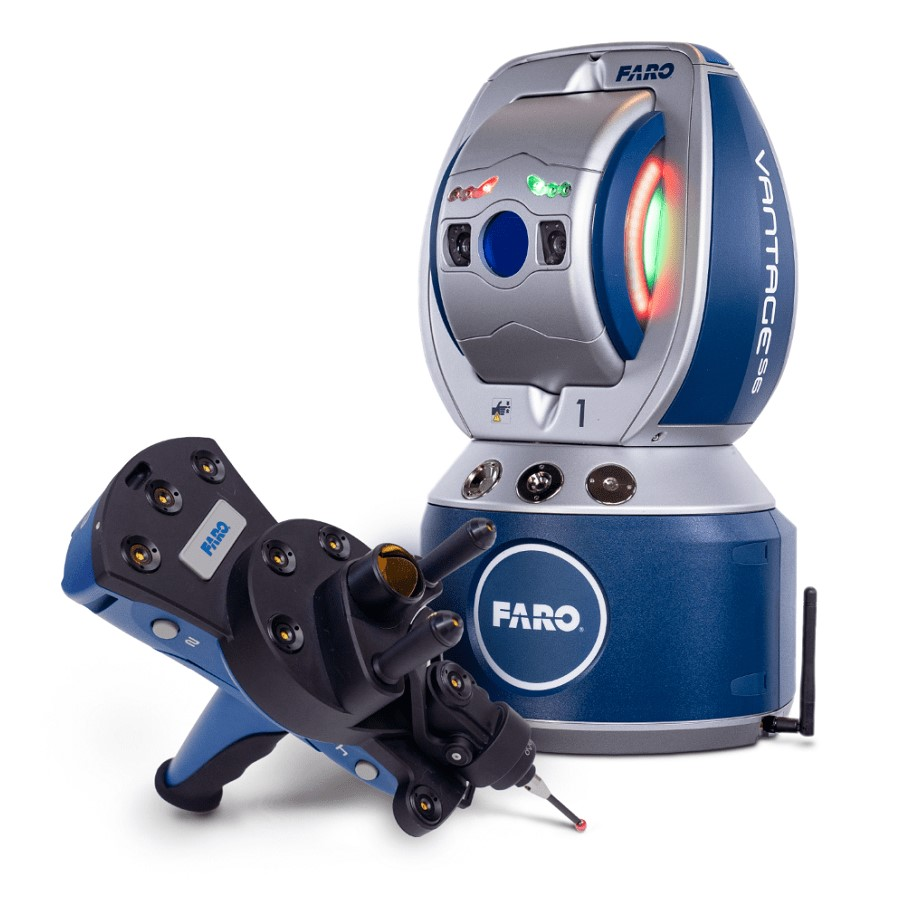
\includegraphics[width=\textwidth]{images/faro-probe.jpg}
          \caption*{\faro Vantage \newline Laser Tracker}
        \end{figure}
      \end{column}
    \end{columns}
  \end{frame}
  \begin{frame}{Problem Description}
    \faro is investing heavily in machine learning. 

    There is a need for algorithm training tools that integrate into \faro codebase.

    This project focuses on demonstrating successful usage of these tools with \faro software.

    We attempt to improve a point cloud alignment function within CAM2\textsuperscript{\textregistered}.

    This function is time expensive and hard to optimize manually.
  \end{frame}
  \begin{frame}{Point Cloud Alignment Function}
    \begin{columns}
      \begin{column}{0.55\textwidth}
        \begin{figure}
        \centering
        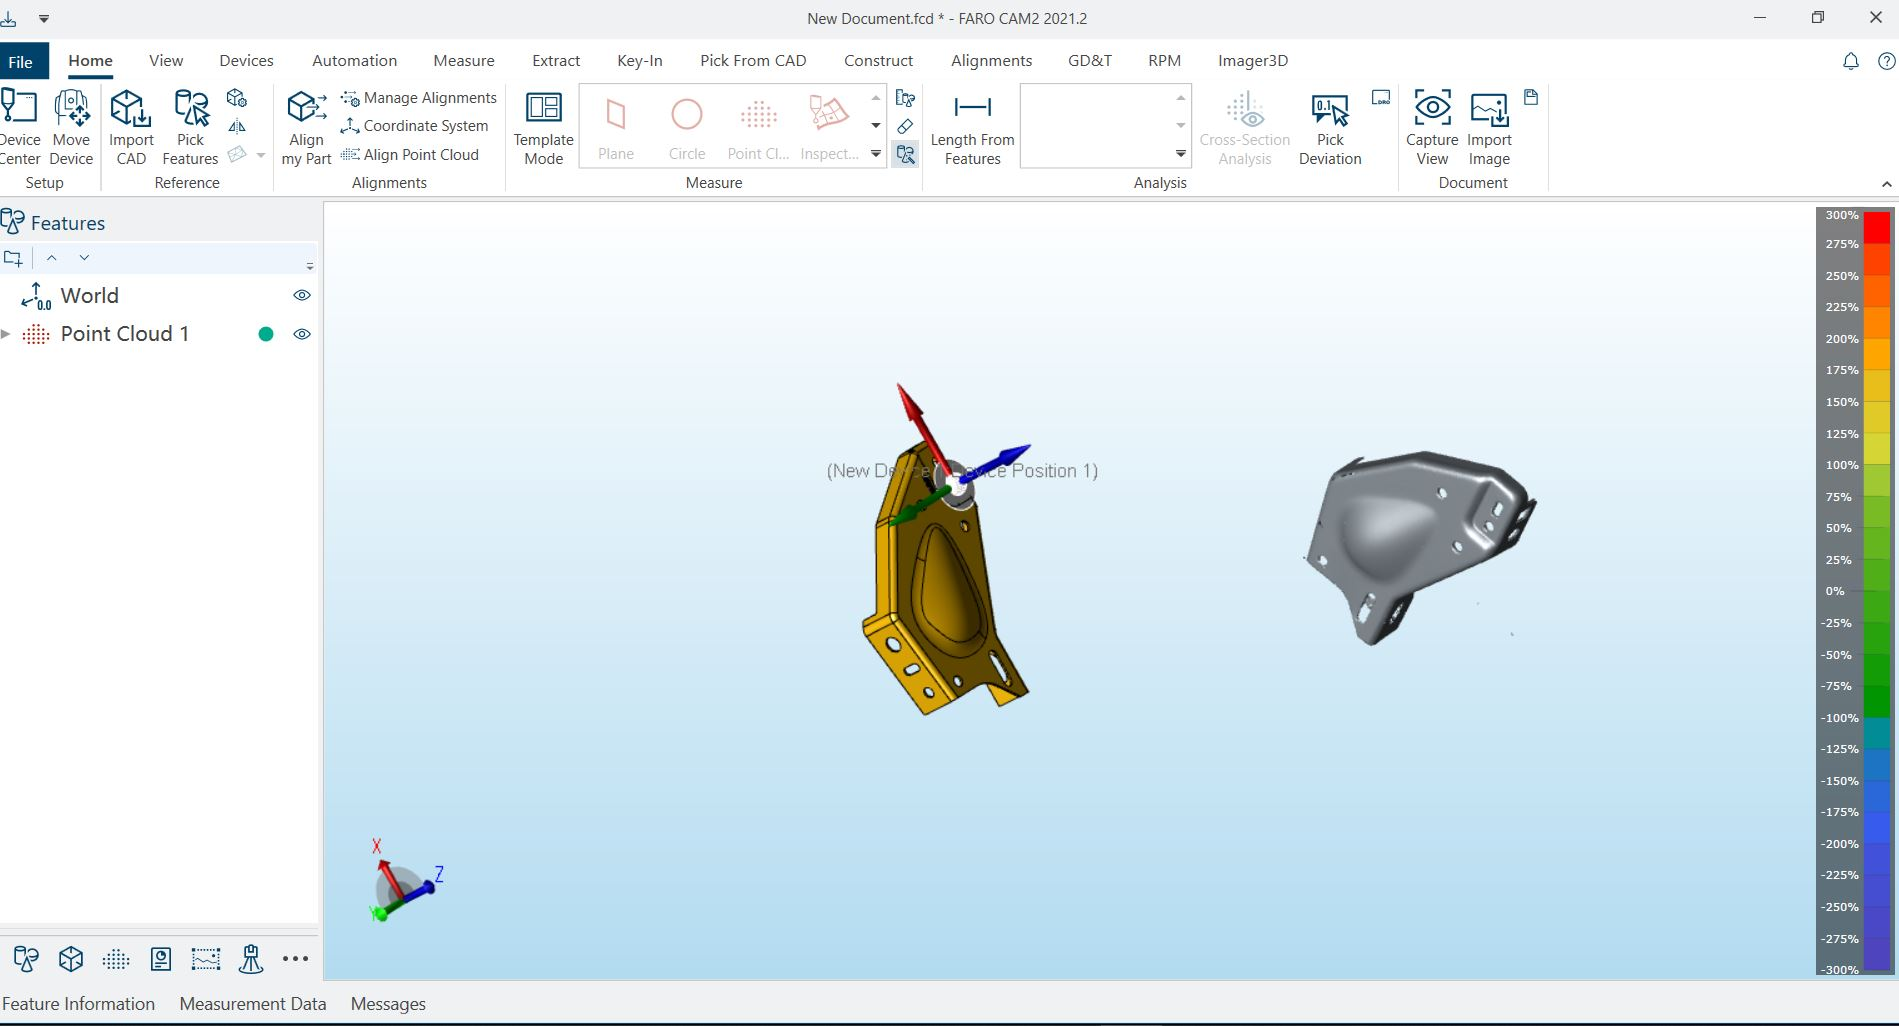
\includegraphics[width=\textwidth]{images/unaligned.png}
        \end{figure}
      \end{column}
      \begin{column}{0.55\textwidth}
        \begin{figure}
        \centering
        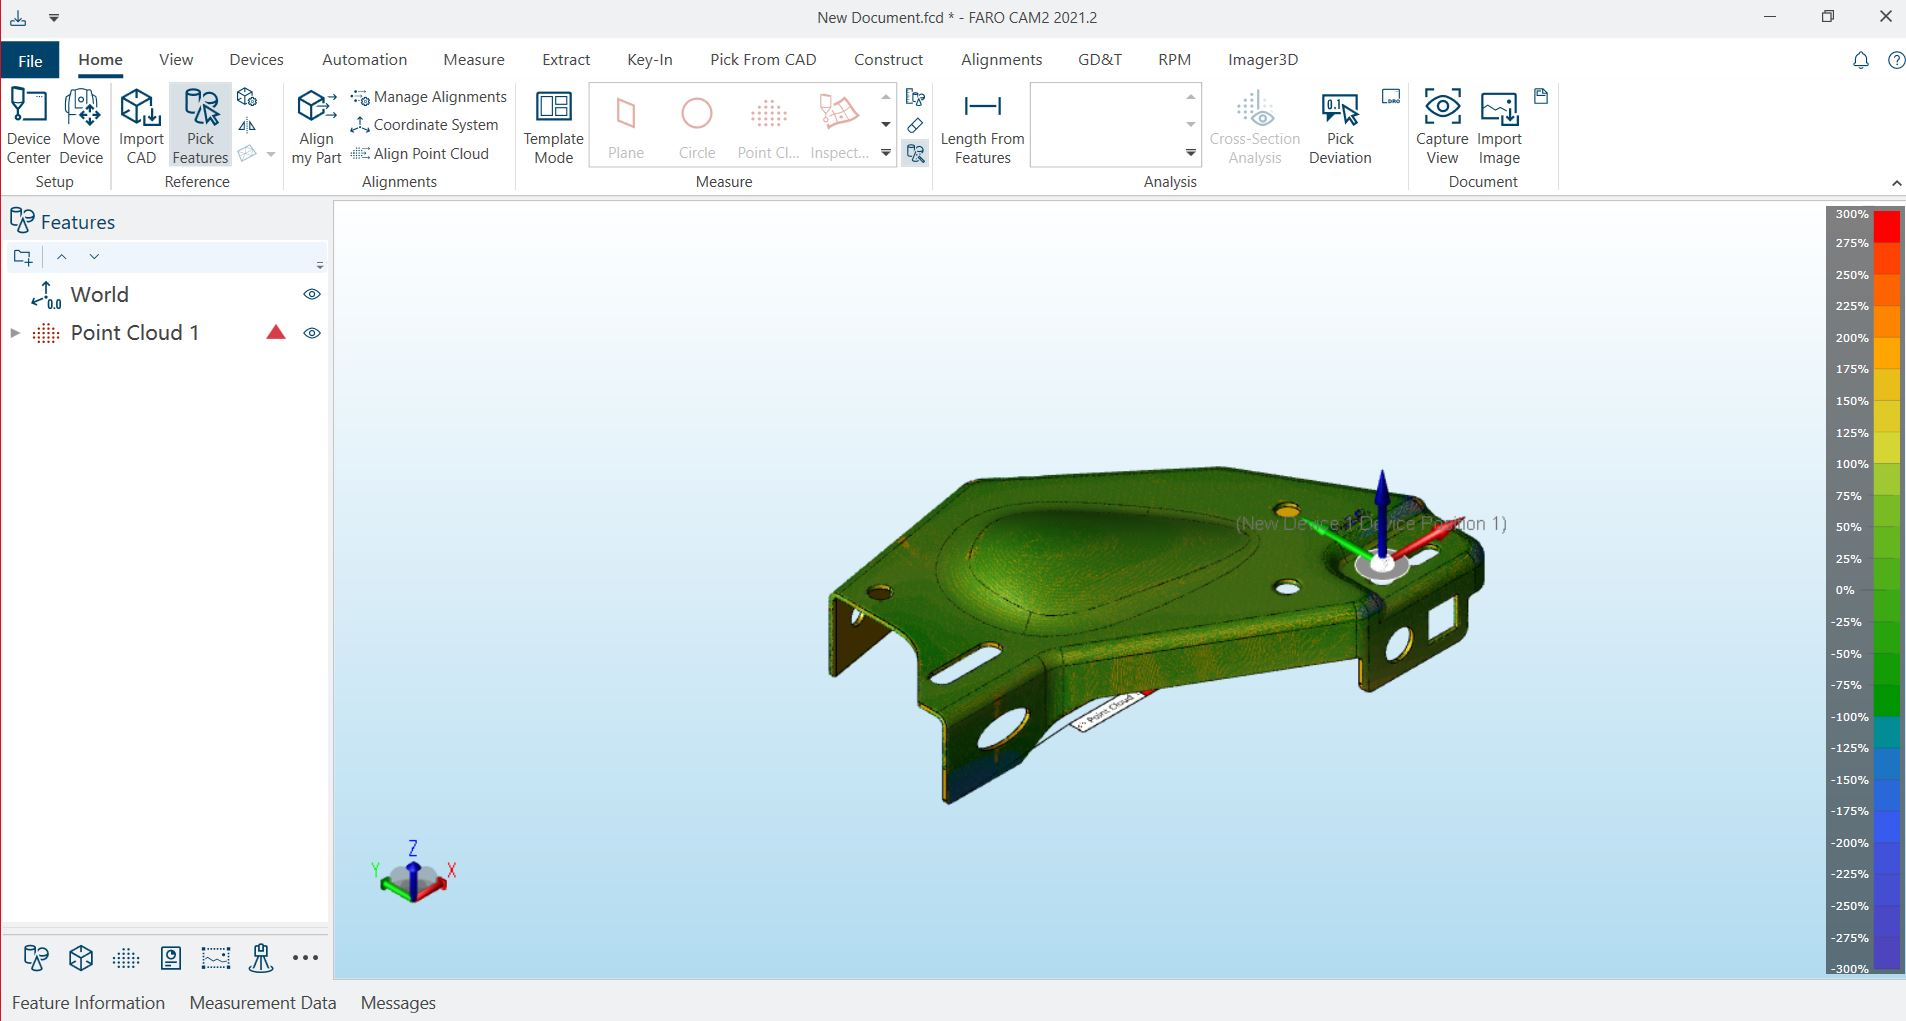
\includegraphics[width=\textwidth]{images/aligned.png}
        \end{figure}
      \end{column}
    \end{columns}
  \end{frame}
  \begin{frame}{Objectives}
    The objective of this internship was to create a solution for hyper parameter optimization (HPO) in software solutions developed by \farons. These main goals were defined:
    \begin{itemize}
      \item Develop 3 algorithm training solutions
      \item Develop meaningful unit tests for these solutions
      \item Integrate the solutions into pre-existing software
      \item Demonstrate value by solving real world issues in CAM2\textsuperscript{\textregistered}
    \end{itemize}
  \end{frame}

  \section{State of the Art}
  \subsection{Related Works}
  \begin{frame}{Related Works}
    We have explored the existing field of hyper parameter optimization. 

    This field has a long history. Its contributors have produced a variety of solutions for the problem at hand. 

    These solutions can be divided into 2 categories: black-box optimization and multi-fidelity optimization.
  \end{frame}
  \begin{frame}{Related Works}
    \begin{figure}
          \centering
          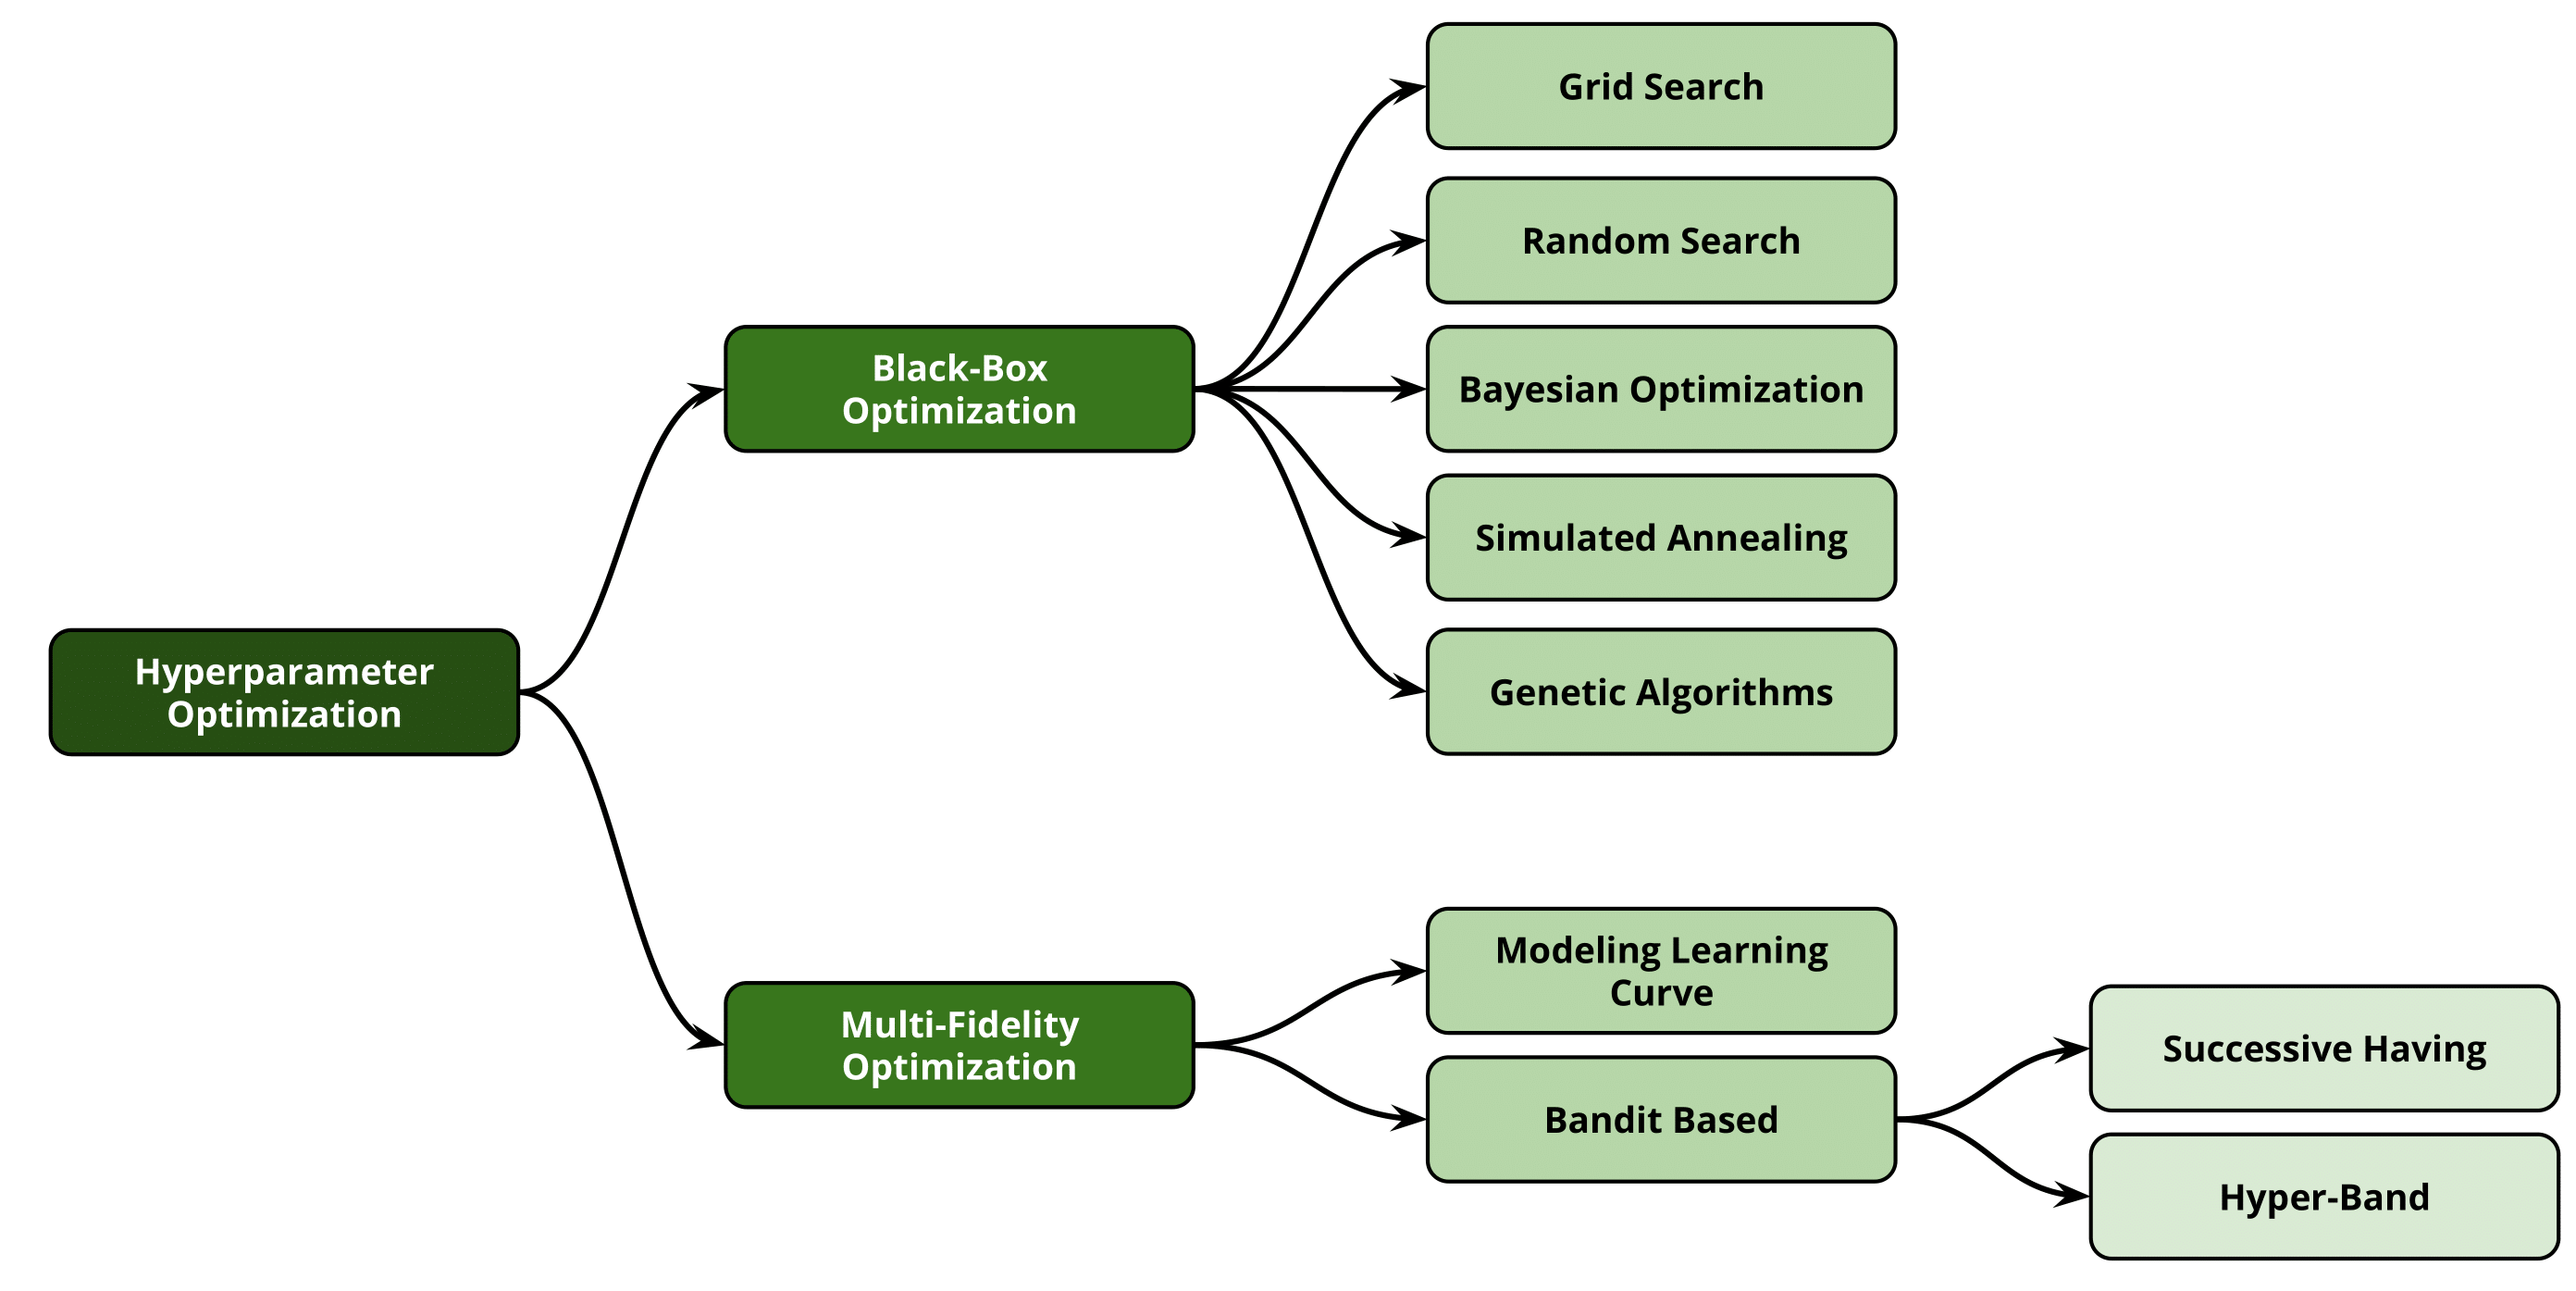
\includegraphics[width=\textwidth]{images/state_art-taxonomy_optimizers.png}
          \caption*{A Taxonomy for Hyper-parameter Optimization Techniques (Elshawi, Maher, \& Sakr, 2019)}
        \end{figure}
  \end{frame}
  \begin{frame}{Black-Box Optimization Algorithms}
    Black-box optimization algorithms treat the problem function as a black-box (a process that is not analytically available).
    \begin{itemize}
      \item{Grid Search}
      \item{Random Search}
      \item{Bayesian Optimization}
    \end{itemize}
  \end{frame}
  \begin{frame}{Multi-Fidelity Optimization Algorithms}
    Multi-fidelity optimization algorithms focus on decreasing the evaluation cost of a given function by combining cheap low-fidelity and expensive high-fidelity evaluations.
    \begin{itemize}
          \item{HyperBand}
          \item{Bayesian Optimization and HyperBand (BOHB)}
    \end{itemize}
  \end{frame}

  \subsection{Existing Technologies}
  \begin{frame}{Existing Technologies}
    HPO is an important part of machine learning development. 

    This is usually implemented in a integrated machine learning development framework. 

    To comply with the scope of this project, we have researched frameworks that are model agnostic, written in Python and able to work with black-box functions.

    We also specify other important software tools options.
  \end{frame}
  \begin{frame}{Hyper Parameter Optimization}
    \begin{figure}[ht]
      \centering
      \begin{tabular}{cccc}
        \subfloat[DeterminedAI]{
\includegraphics[width=2cm]{images/determined.png}} &
        \subfloat[AutoML]{
\includegraphics[width=2cm]{images/automl.png}} &
        \subfloat[HyperOpt]{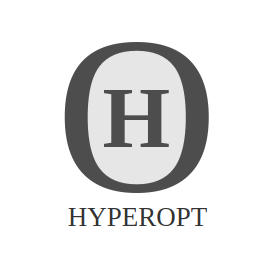
\includegraphics[width=2cm]{images/hyperopt.png}} &
        \subfloat[Scikit Learn]{
\includegraphics[width=2cm]{images/scikit.png}} \\
        \subfloat[Ray Tune]{
\includegraphics[width=2cm]{images/ray_tune.png}} &
        \subfloat[Amazon Sagemaker]{
\includegraphics[width=2cm]{images/sagemaker.png}} &
        \subfloat[Google HyperTune]{
\includegraphics[width=2cm]{images/google_ai.png}}
      \end{tabular}
      \caption*{Hyper Parameter Optimization Libraries}
    \end{figure}
  \end{frame}
  \begin{frame}{Virtualization}
    \begin{figure}[hb]
      \centering
      \begin{tabular}{ccc}
      \subfloat[Docker/Moby]{
\includegraphics[width = 2cm]{images/Moby-logo.png}} &
      \subfloat[Kubernetes]{
\includegraphics[width = 2cm]{images/k8s-logo.png}} &
      \subfloat[VMware Workstation]{
\includegraphics[width = 2cm]{images/vmworkstation.png}}
      \end{tabular}
      \caption*{Commercial Virtualization Products}
    \end{figure}
  \end{frame}
  \begin{frame}{Machine Learning Data Visualization}
    \begin{figure}[ht]
      \centering
      \begin{tabular}{ccc}
      \subfloat[Weights and Biases]{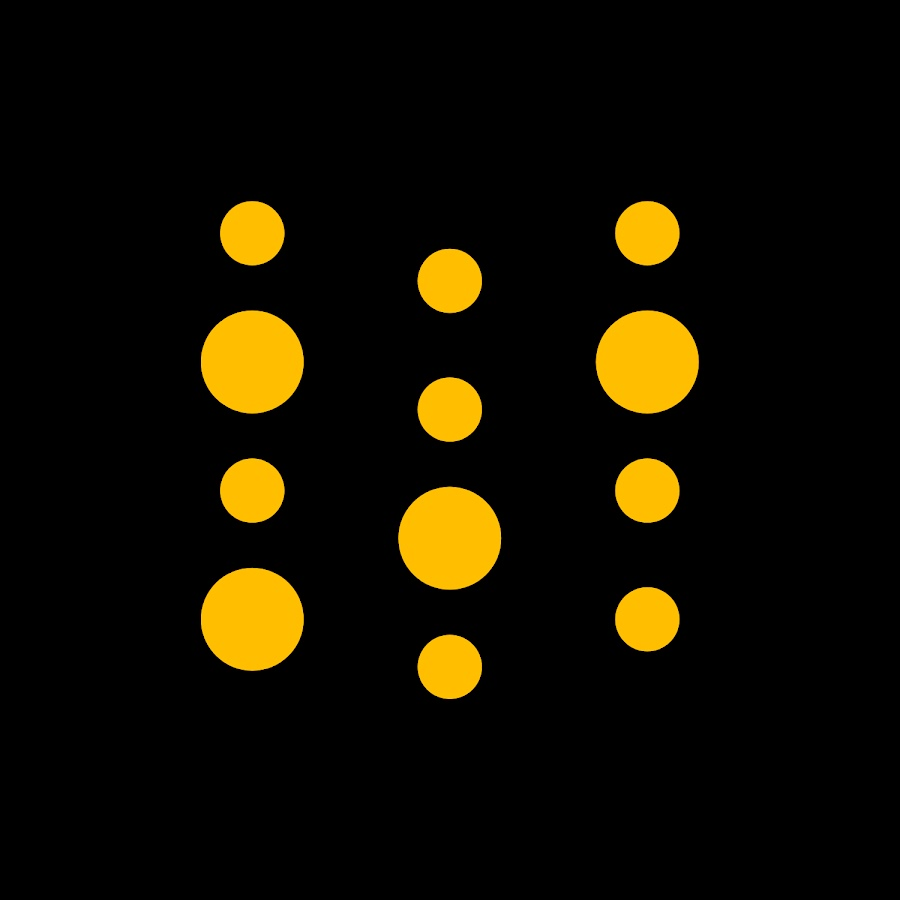
\includegraphics[width = 2cm]{images/wandb.png}} &
      \subfloat[TensorBoard]{
\includegraphics[width = 2cm]{images/tensorboard.png}} &
      \subfloat[Neptune]{
\includegraphics[width = 2cm]{images/neptune.png}} \\
      \subfloat[Guild AI]{
\includegraphics[width = 2cm]{images/guildai.jpg}} &
      \subfloat[Comet]{
\includegraphics[width = 2cm]{images/coemt.png}}
      \end{tabular}
      \caption*{Machine Learning Data Visualization Tools}
    \end{figure}
  \end{frame}

  \section{Analysis}
  \begin{frame}{Domain}
    \begin{figure}
      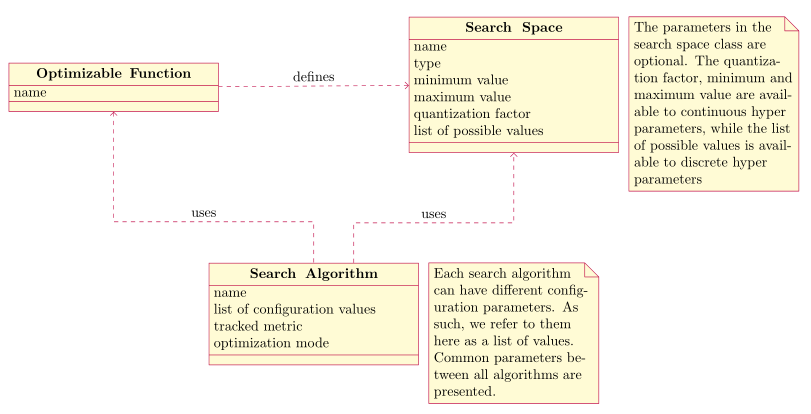
\includegraphics[width=\textwidth]{images/domain_model.png}
      \caption*{Domain Model}
    \end{figure}
  \end{frame}
  \begin{frame}{Requirements}
    The requirements for this project followed the FURPS+ model.

    MAYBE ADD IMAGE HERE
  \end{frame}
  \begin{frame}{Functionality}
    \begin{itemize}
      \item A privileged developer can integrate new HPO algorithms into the framework
      \item A developer can define all necessary information to allow the optimization pipeline to run (hyper parameter definitions, objective function instantiation, algorithm selection, etc.)
      \item A developer can obtain information during and at the end of the optimization process regarding said process
      \item A developer can run the optimization pipeline.
    \end{itemize}
  \end{frame}
  \begin{frame}{Usability}
    \begin{itemize}
      \item There should be comprehensive documentation on how the system functions and how a user interacts with it
      \item There should be pre-existing examples of usage of the system.
    \end{itemize}
  \end{frame}
  \begin{frame}{Reliability}
    \begin{itemize}
      \item The system should be able to recover from external failures (eg.\ issues with CAM2\textsuperscript{\textregistered})
      \item The system should be able to save its state in order to allow for interruptions in the execution.
    \end{itemize}
  \end{frame}
  \begin{frame}{Performance}
    \begin{itemize}
      \item The software should be faster than the CAM2\textsuperscript{\textregistered}'s endpoints it accesses
      \item The software should be efficient in such a way that it does not interfere with the CAM2\textsuperscript{\textregistered} software
      \item The system should consume as little resources as possible, allowing for it to be run directly in the developer's issued laptop, without interfering with other programs.
    \end{itemize}
  \end{frame}
  \begin{frame}{Supportability}
    \begin{itemize}
      \item The developed code should include meaningful testing, insuring the correct operation of the software
      \item The developed system should allow for extending its usage to new algorithms and optimizable functions
      \item The developer should be able to define their preferred configuration when executing the software
      \item The software should be installable in any of \farons's issued laptop easily.
    \end{itemize}
  \end{frame}
  \begin{frame}{Design Constraints}
    \begin{itemize}
      \item The developed application must be implemented in Python.
    \end{itemize}
  \end{frame}
  \begin{frame}{Implementation Constraints}
    \begin{itemize}
      \item The developed application must executed with minimal resource allocation (with regards to CPU usage and RAM allocation)
      \item The developed application must be able to execute in a Windows environment.
    \end{itemize}
  \end{frame}
  \begin{frame}{Interface Constraints}
    \begin{itemize}
      \item The optimization pipeline must allow communication with the CAM2\textsuperscript{\textregistered} integrated web server
      \item Said communication must be executed through HTTP, using pre existing endpoints.
    \end{itemize}
  \end{frame}
  \begin{frame}{Physical Constraints}
    \begin{itemize}
      \item The developed system should be executed in the same network as the CAM2\textsuperscript{\textregistered} integrated web server.
    \end{itemize}
  \end{frame}

  \section{Design}
  \begin{frame}{Design}
    The developed system was designed using the C4 model, a technique for modelling the architecture of software systems. 
    This system documents a software system by splitting it into multiple levels.
    \begin{figure}[H]
      \centering
      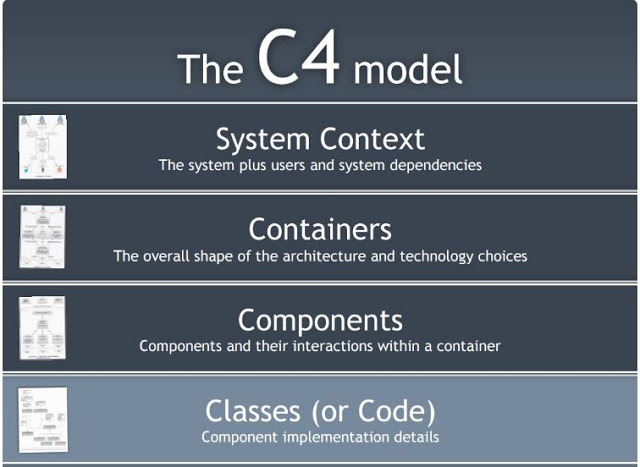
\includegraphics[width=0.5\textwidth]{images/c4.jpg}
      \caption*{C4 Model}
    \end{figure}
  \end{frame}
  \begin{frame}{Context}
    \begin{figure}[H]
      \centering
      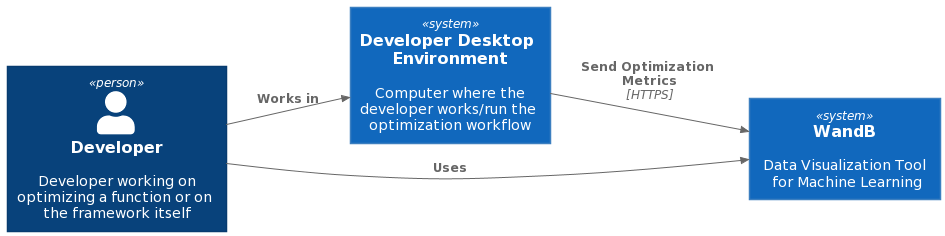
\includegraphics[width=\textwidth, keepaspectratio]{images/c1_new.png}
      \caption*{Level 1: Container diagram}
    \end{figure}
  \end{frame}
  \begin{frame}{Containers}
    \begin{figure}[H]
      \centering
      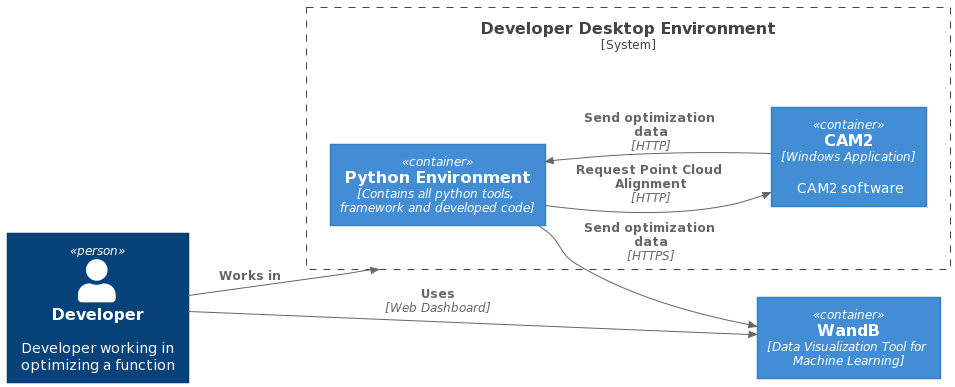
\includegraphics[width=\textwidth, keepaspectratio]{images/c2_new.png}
      \caption*{Level 2: Container diagram}
    \end{figure}
  \end{frame}
  \begin{frame}{Components}
    \begin{figure}[H]
    \centering
    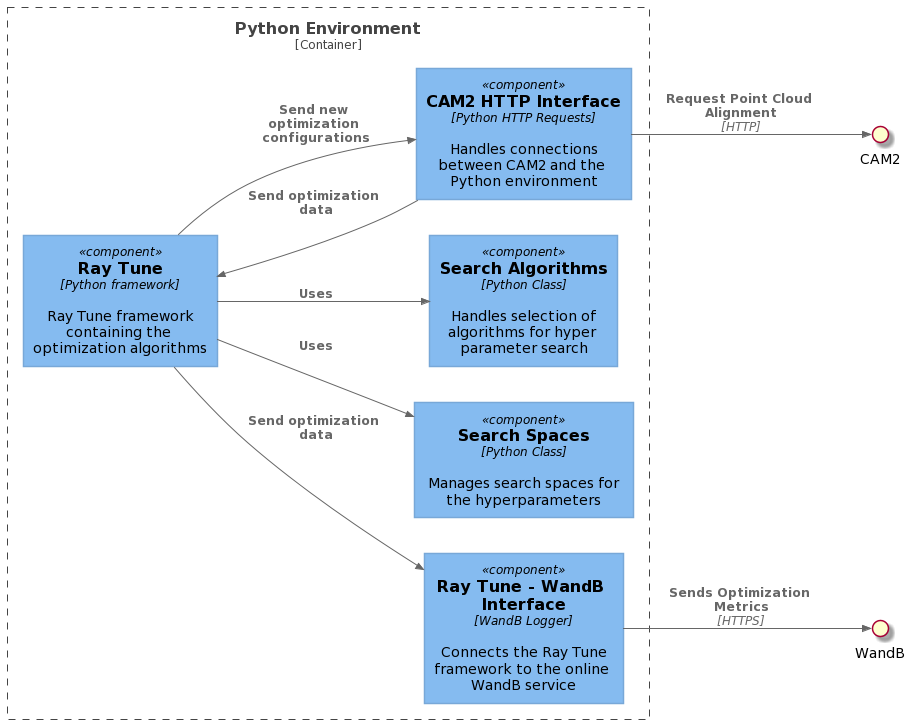
\includegraphics[width=0.8\textwidth]{images/c3_python.png}
    \caption*{Level 3: Python Environment Component Diagram}
    \label{fig:l3_python}
    \end{figure}
  \end{frame}
  \begin{frame}{Components}
    \begin{figure}[H]
    \centering
    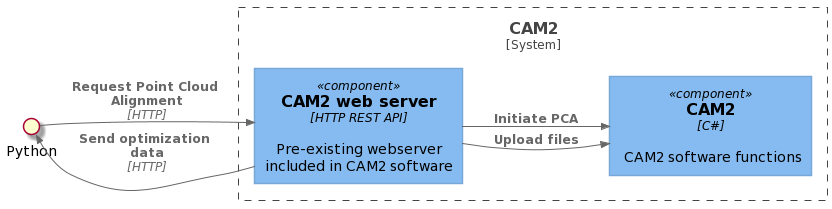
\includegraphics[width=\textwidth]{images/c3_cam2.png}
    \caption*{Level 3: CAM2 Component Diagram}
    \label{fig:l3_cam2}
    \end{figure}
  \end{frame}
  \begin{frame}{Components}
    \begin{figure}[H]
    \centering
    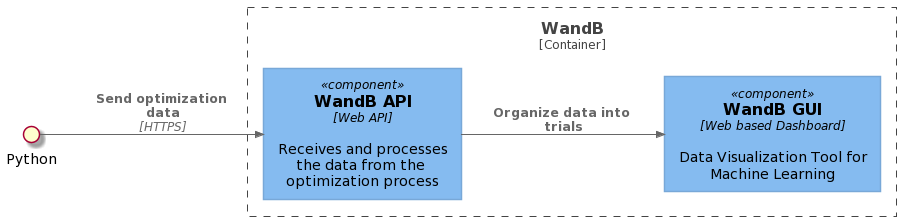
\includegraphics[width=\textwidth]{images/c3_wandb.png}
    \caption*{Level 3: WandB Component Diagram}
    \label{fig:l3_wandb}
    \end{figure}
  \end{frame}

  \section{Implementation}
  \begin{frame}{Evaluation}
    \begin{figure}
      \centering
      \href{https://bit.ly/3yIZQC4}{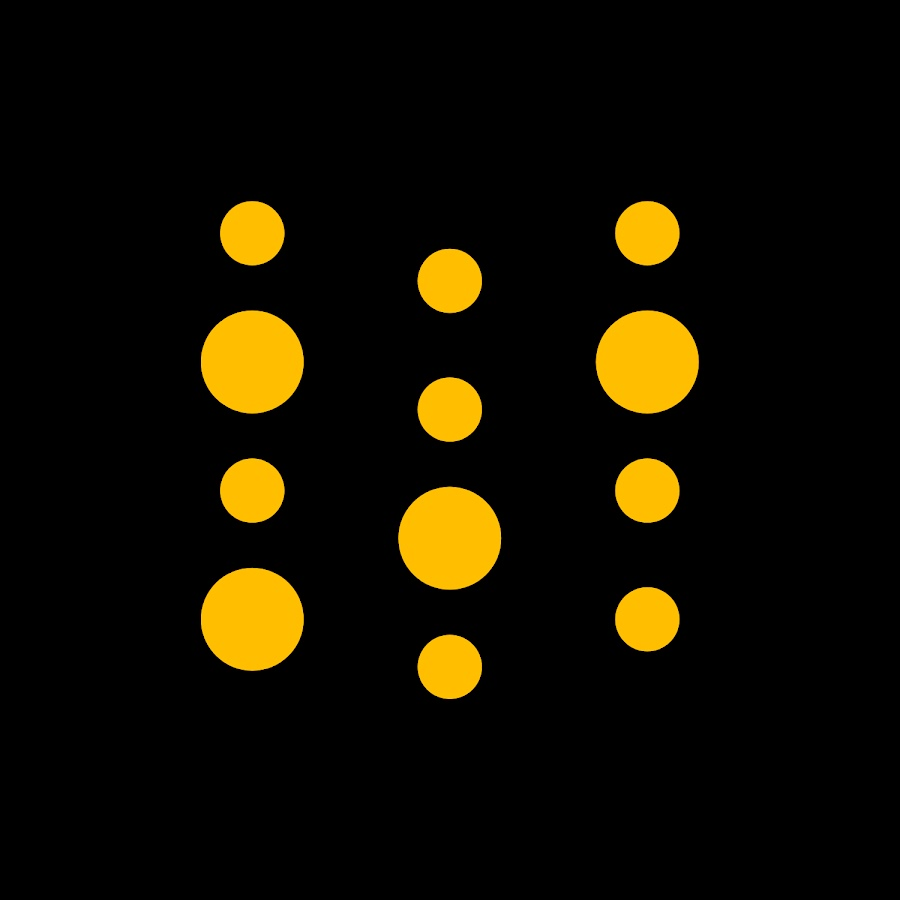
\includegraphics[width=0.6\textwidth]{images/wandb.png}}
    \end{figure}
  \end{frame}

  \section{Conclusion}
  \begin{frame}{Objectives}
    From the initially defined objectives, we can say each of these goals was achieved with various degrees of success. 
    \begin{itemize}
      \item Developed a solution that includes a wide range of HPO algorithms to use, most of which are academically tested and state of the art.
      \item Developed tests for the developed infrastructure behind the solution.
      \item Successfully integrated the solution into CAM2.
      \item Demonstrated real world value to the team at \farons.
    \end{itemize}
  \end{frame}
  \begin{frame}{Limitations and Future Work}
    First and foremost, the non-parallel nature of CAM2\textsuperscript{\textregistered} limits the developed solution. In the future, this issue can be overcome by using networked computers, where we can run CAM2\textsuperscript{\textregistered} in a parallel way.

    Furthermore, the hyper parameters exposed through the CAM2\textsuperscript{\textregistered} API are not complete. As such, we cannot reliably validate the current configuration of these hyper parameters and in future work exposing more parameters and optimizing these as well may yield better results.

    Finally, after analysing the results, we believe that the point cloud that is provided to the CAM2\textsuperscript{\textregistered} software may be an important factor to the performance of the PCA function. In the future, further refining the data set, separating and finding common features between each separate subset may allow for even better optimization.
  \end{frame}
  \begin{frame}{Final Remarks}
    In retrospect, the author is overwhelmingly satisfied with the project, its results and the experience provided by \farons 's Research Department.

    Integrating a variety of systems and services has provided the author with valuable insight into API management. 

    The tight connection with ML and AI through the HPO algorithms also enabled the author to understand this field of research more thoroughly.

    The introduction of new concepts was a novel experience, but with proper research the author was able to understand the introduced concepts.

    Overall, the author has found this internship to be a positive academically and professionally and is thankful to all stakeholders in this project.
  \end{frame}


\end{document}
